\chapter{Постановка задачи} \label{chapt2}

\section{Содержательная} \label{sect2_1}
\textbf{Дано: } 

Изображение или видеопоток, с камеры устройства. 

\textbf{Требуется: } 

Определить, присутствует ли на кадре собака и вернуть информацию о позе собаки в данный момент среди следующих классов $Y \in$ (\emph{Стоит,  Сидит,  Лежит}).

Требования к изображению и видеопотоку, которые идут на вход классификатору изображений (далее $C$). 

\begin{itemize}
    \item На изображении должна присутствовать собака
    \item Размер изображения больше 300 пикселей по короткой стороне
    \item Изображение цветное, трёхканальное
    \item Фокус изображения должен быть на собаке в кадре
\end{itemize}

Собака в кадре должна быть:
\begin{itemize}
    \item Видна целиком
    \item Ничем не загорожена, даже частично
    \item На кадре находиться одна
    \item 4 лапы и голова собаки должны быть видны целиком и не быть загорожены
    \item Занимать более 20\% кадра по высоте и по ширине
    \item Собака должна находится в одной из поз, среди массива классов $Y$
 \end{itemize}
 
Камера относительно собаки:
\begin{itemize}
    \item Находится на расстоянии более 2м
    \item Смотрит на собаку на уровне глаз либо выше, но не сверху.
\end{itemize}

Если на кадре не выполняются указанные условия, определять позу собаки не требуется.

Требования к полученной системе:
\begin{itemize}
    \item Точность классификации $Precision_{lim}$ должна быть выше 90\% для каждого из классов
    \item Частота работы системы $\nu_{lim}$ превышает 1Гц.
\end{itemize}


\section{Математическая}\label{sect2_2}

В данной работе решается задача классификации изображений со следующей формулировкой. 

Имеется видеопоток, который подаётся в систему с частотой $\nu$, измеряемой в Герцах. Необходимо произвести классификацию изображений из видеопотока по заранее известному $N$ количеству классов и вернуть сообщение с номером класса или ответить что изображение не подходит под условия задачи $C$, которые указаны в п.\ref{sect2_1}. 

Допустимо пропускать некоторые изображения, если частота видеопотока превышает частоту работы системы, но частота ответов должна превышать $\nu_{lim}$. 

Изображения, которые не подходят под условия задачи $C$, классифицировать не требуется, но требуется вернуть ответ о том, что они не подходят. 

Допустимо классифицировать изображения с ошибкой, но точность классификации должна быть не меньше $Precision_{lim}$ для конечного набора классифицированных изображений $X$.

В задачи классификации изображений, объекты — это фотографии. Формальная постановка задачи классификации изображений:

$ V = \begin{pmatrix} 
             I_1, & I_2, & ..., & I_n 
      \end{pmatrix}
$
~— множество изображений. 

$ Y = \begin{pmatrix}
                  y_1, & y_2, & ..., & y_n 
      \end{pmatrix}
$
~— конечное множество меток классов.

$y^{*} : V \rightarrow Y$ — неизвестная целевая зависимость, значения которой известны только на объектах конечной обучающей выборки 
\[ D_m = 
        \begin{pmatrix}
             (I_1, y_1), & ..., & (I_m, y_m)
        \end{pmatrix}
\].

Требуется построить алгоритм $a : V \rightarrow Y$ , способный классифицировать объект $I \in V$, который отвечает условиям $C$.


\subsection{Структура входных данных}
Исходными данными в задаче является конечная последовательность кадров, полученная с видеоряда  камеры телефона.

\begin{equation}
    V = \begin{pmatrix}
                I_1, & I_2, & ..., & I_3
        \end{pmatrix}
\end{equation}          

Каждый кадр, или изображение из этого видеоряда является трёхмерной матрицей с количеством столбцов  $h$, количеством строк $w$ и глубиной 3 (красный, зелёный и синий цветовые каналы). 

\begin{equation} 
I =    \begin{pmatrix} 
            \begin{bmatrix}
            r_{1,1} & g_{1,1} & b_{1,1}\\
            r_{1,2} & g_{1,2} & b_{1,2}\\
            ...\\
            r_{1,w} & g_{1,w} & b_{1,w}\\
            \end{bmatrix}\\
            \begin{bmatrix}
            r_{2,1} & g_{2,1} & b_{2,1}\\
            r_{2,2} & g_{2,2} & b_{2,2}\\
            ...\\
            r_{2,w} & g_{2,w} & b_{2,w}\\
            \end{bmatrix}\\
            ...\\
            \begin{bmatrix}
            r_{h,1} & g_{h,1} & b_{h,1}\\
            r_{h,2} & g_{h,2} & b_{h,2}\\
            ...\\
            r_{h,w} & g_{h,w} & b_{h,w}\\
            \end{bmatrix}\\ 
        \end{pmatrix}
\end{equation}

\subsection{Структура выходных данных}\label{input_struct}
В работе требуется построить оператор $F$  который бы заполнял описанную структуру исходя из поставленной задачи:

\begin{equation}
    F:V \rightarrow RS
\end{equation}

Результаты работы алгоритма заносятся в объект «Состояние собаки»:

\begin{equation}
    RS = \begin{pmatrix}
            Prob, & Loc, & Breed, & Pose 
        \end{pmatrix}
\end{equation}

В этом объекте

$Prob$ - число, вероятность того что на кадре присутствует собака.

$Loc$ - вектор, содержащий информацию об ограничивающей рамке собаки. Состоит из следующих значений:
\[
Loc =   \begin{pmatrix}
                x_{min}, & x_{max}, & y_{min}, & y_{max} 
        \end{pmatrix}
\]

$Breed$ - Вектор для вероятностей принадлежности изображения, внутри $loc$ к каждому из 120 классов пород собаки.

$Pose$ - Вектор вероятности принадлежности изображения внутри $loc$ к каждой из 3 классов поз собаки.

\subsection{Алгоритм решения поставленной задачи}\label{algorithm}
\begin{figure}[ht] 
  \center
  \includegraphics [width=\textwidth*2/3] {flowchart}
  \caption{Функциональная схема поставленной задачи} 
  \label{img:flowchart}  
\end{figure}
Для того, чтобы гарантировать исполнение условий, указанных в содержательной постановке задачи, используется предобученная нейронная сеть по сегментации изображений MaskRCNN \cite{maskrcnn}, она указана на схеме (рисунок \ref{img:flowchart}) как детектор объектов. Она получает на вход изображение $I$ и возвращает маску объектов $M$, находящихся на ней.

\[
I \rightarrow M
\]

$I$ - Изображение размером 224 пикселя по высоте, 224 пикселя по ширине, обладающее тремя цветовыми каналами $R, G, B$

$M$ - Маска - это бинарное изображение, по высоте и ширине совпадающее с входным изображением, где наличие сигнала (белый цвет) говорит о наличии объекта на кадре. Наглядно это показано на рисунке \ref{img:mask}.
\begin{figure}[ht] 
  \center
  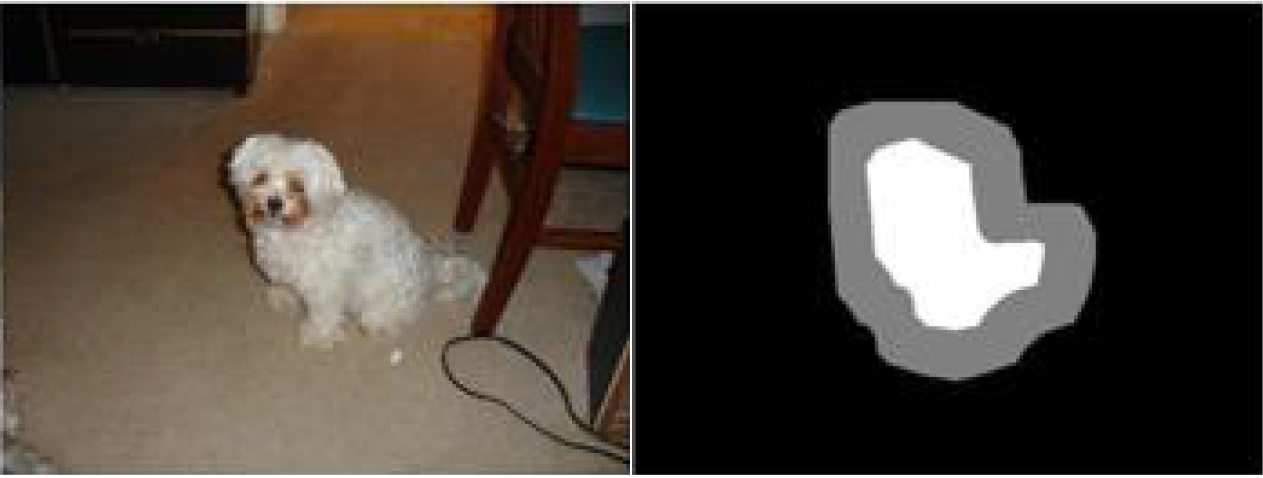
\includegraphics [width=\textwidth*2/3] {mask}
  \caption{Изображение собаки и маска собаки для этого изображения} 
  \label{img:mask}  
\end{figure}

Если на маске собаки несколько замкнутых фигур, значит, на кадре больше одной собаки. Если маска собаки пуста, значит на кадре собак нет. Эти две простые проверки сильно увеличивают качество предсказания нейронной сети сети. 

Помимо этих проверок, маска позволяет убрать ненужную часть кадра, уменьшая шанс того, что нейронная сеть ошибётся.

Обрезанное изображение по маске собаки передаётся далее в нейронную сеть для классификации непосредственно позы собаки. На схеме в рисунке \ref{img:flowchart} она указана как классификатор позы собаки. Для этого используется MobileNet v2\cite{mobilenet}. Изменения от оригинальной статьи только в так называемой «голове» классификации и размере входного изображения. Визуально архитектура представлена на рисунке \ref{img:NN_arch} 

\begin{figure}[ht] 
  \center
  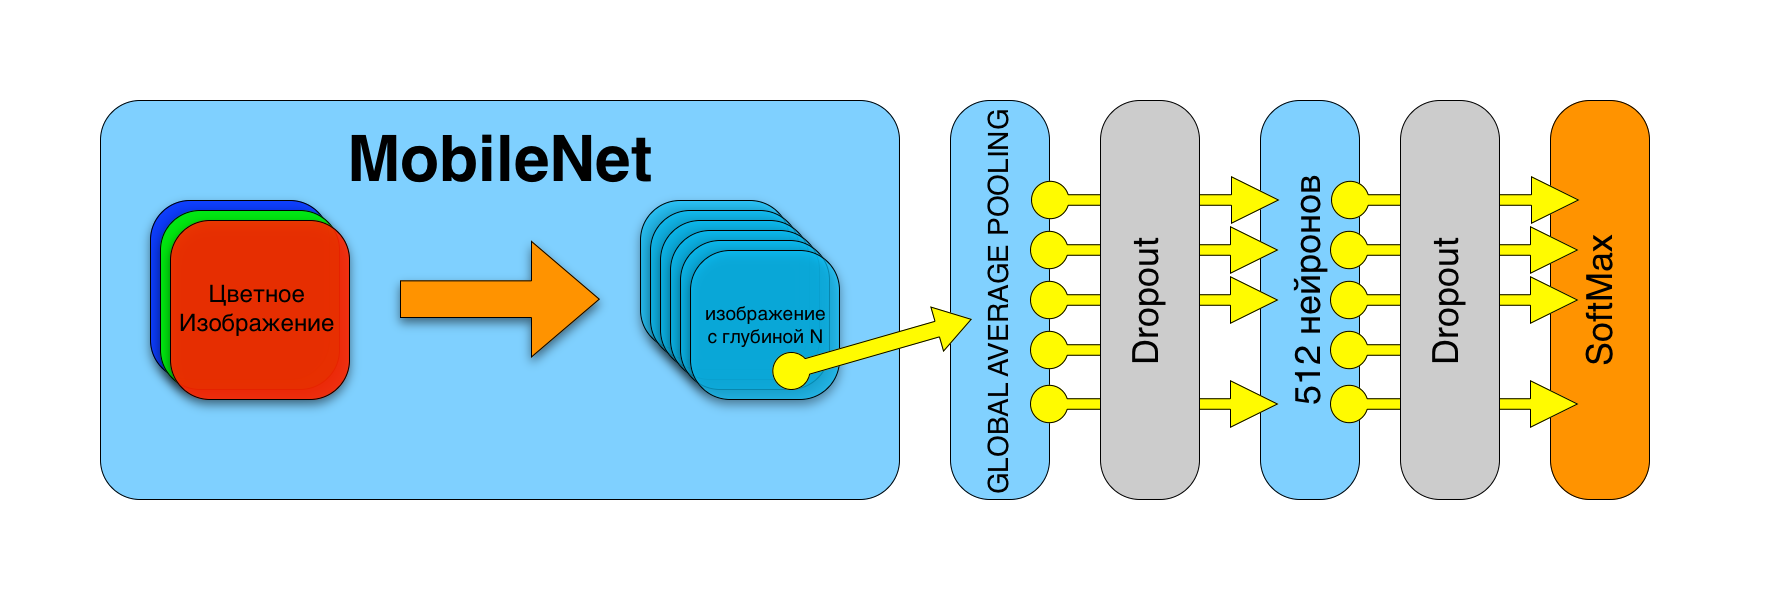
\includegraphics [width=\textwidth] {NN_arch}
  \caption{Архитектура используемой нейронной сети} 
  \label{img:NN_arch}  
\end{figure}

Её характеристики следующие:

\begin{itemize}
    \item Входное изображение I обладает размерностью 96 пикселей по ширине и высоте и 3 цветовыми каналами
    \item Свёрточные слои нейронной сети MobileNet V2\cite{mobilenet}, без "головы".
    \item Global Average Pooling - последняя карта активации(3-мерный тензор $T$ с размерностью $\{x_{d1}, y_{d2}, z_{d3}\}$) преобразуется в плоский вектор $X$ с длинной $d_3$. Каждый слой превращается в одно число - среднее по слою. Это позволяет нейронной сети быть инвариантной к размеру входного изображения.
    
    \[ X_i = \dfrac{1}{d_1*d_2}\sum_{j=0}^{j=d_1}\sum_{k=0}^{k=d_2}T_{i,j,k} \]
    
    \item Слой DropOut\cite{dropout} - обнуление 20\% разных значений предыдущего слоя
    \item Batch Norm\cite{batchnorm} - нормализация вектора относительно других изображений в мини-партии данных для обучения
    \item Полносвязный слой с 512 нейронами
    \item Функция активации, ReLU
    \item слой DropOut
    \item BatchNorm
    \item Выходной слой $n$ нейронов, по количеству классов. Функция активации softmax.
\end{itemize}

Такая архитектура обусловлена борьбой с переобучением нейронной сети на маленьких объёмах данных. Размер входного изображения удерживается на минимальном уровне - 96 пикселей.

Множественные DropOut и Batch Normalization тоже сильно мешают нейронной сети "зазубрить" датасет, так как они каждый раз немного изменяют выходы предыдущих слоёв.

\subsection{Инструменты и средства разработки}\label{ide}
Программное обеспечение алгоритма распознавания позы собакибыл реализовано на языке программирование Python с помощью библиотеки компьютерного зрения OpenCV, а также библиотеки для обучения нейронных сетей Keras в интегрированной среде разработки PyCharm.

Python - интерпретируемый язык с динамической типизацией общего назначения. Данный язык программирования поддерживает такие парадигмы программирования, как процедурное программирование, объектно-ориентированное программирование и обобщенное программирование. Также он обеспечивает модульность, обработку исключений, трассировку ошибок, абстракцию данных, объявление классов объектов и лямбда-функции.

OpenCV (англ. Open Source Computer Vision Library, библиотека компьютерного зрения с открытым исходным кодом) — библиотека алгоритмов компьютерного зрения, обработки изображений и численных алгоритмов общего назначения с открытым кодом.

Приложение для мобильного телефона разрабатывалось в интегрированной среде разработки XCode с применением библиотек Metal, CoreML и Vision. CoreML является библиотекой для машинного обучения и работы с нейронными сетями для продуктов компании Apple и сделан на базе Metal, который позволяет использовать специализированные инструкции новых процессоров включая Neural Engine, который ускоряет работу с нейронными сетями в несколько раз. В качестве языка для приложения на телефоне использовался Swift 4.2. 